\documentclass[12pt]{scrartcl}


\usepackage{float}

\usepackage[utf8]{inputenc}

\usepackage[T1]{fontenc}

\usepackage{lmodern}

\usepackage[ngerman]{babel}

\usepackage{amsmath}

\usepackage{graphicx}


 

\title{Versuch AP1ph\\ Messung der Elementarladung - Der Milikansche Öltröpfchenversuch}

\author{Frederik Strothmann, Henrik Jürgens}

\date{\today}


\begin{document}


 %deckblatt erstellen

\maketitle
\tableofcontents
\newpage

%einleitung zu dem experiment

\section{Einleitung}

Ein lange bekanntes Quantenphänomen aus dem Bereich der Physik ist die Tatsache, dass es eine kleinste
Ladungseinheit, nämlich die Elementarladung $e$ gibt. Im Jahr 1909 gelang es R. A. MILLIKAN, diese Elementarladung direkt zu messen, indem er die Bewegung mikroskopisch kleiner Öltröpfchen im homogenen Feld eines Plattenkondensators studierte. Dieser Versuch soll wiederholt und ein möglichst genauer Wert für $e$ ermittelt werden.
%versuchsaufbau mit skizze

\section{Versuchsaufbau}

\begin{figure}[H] 
  \centering
    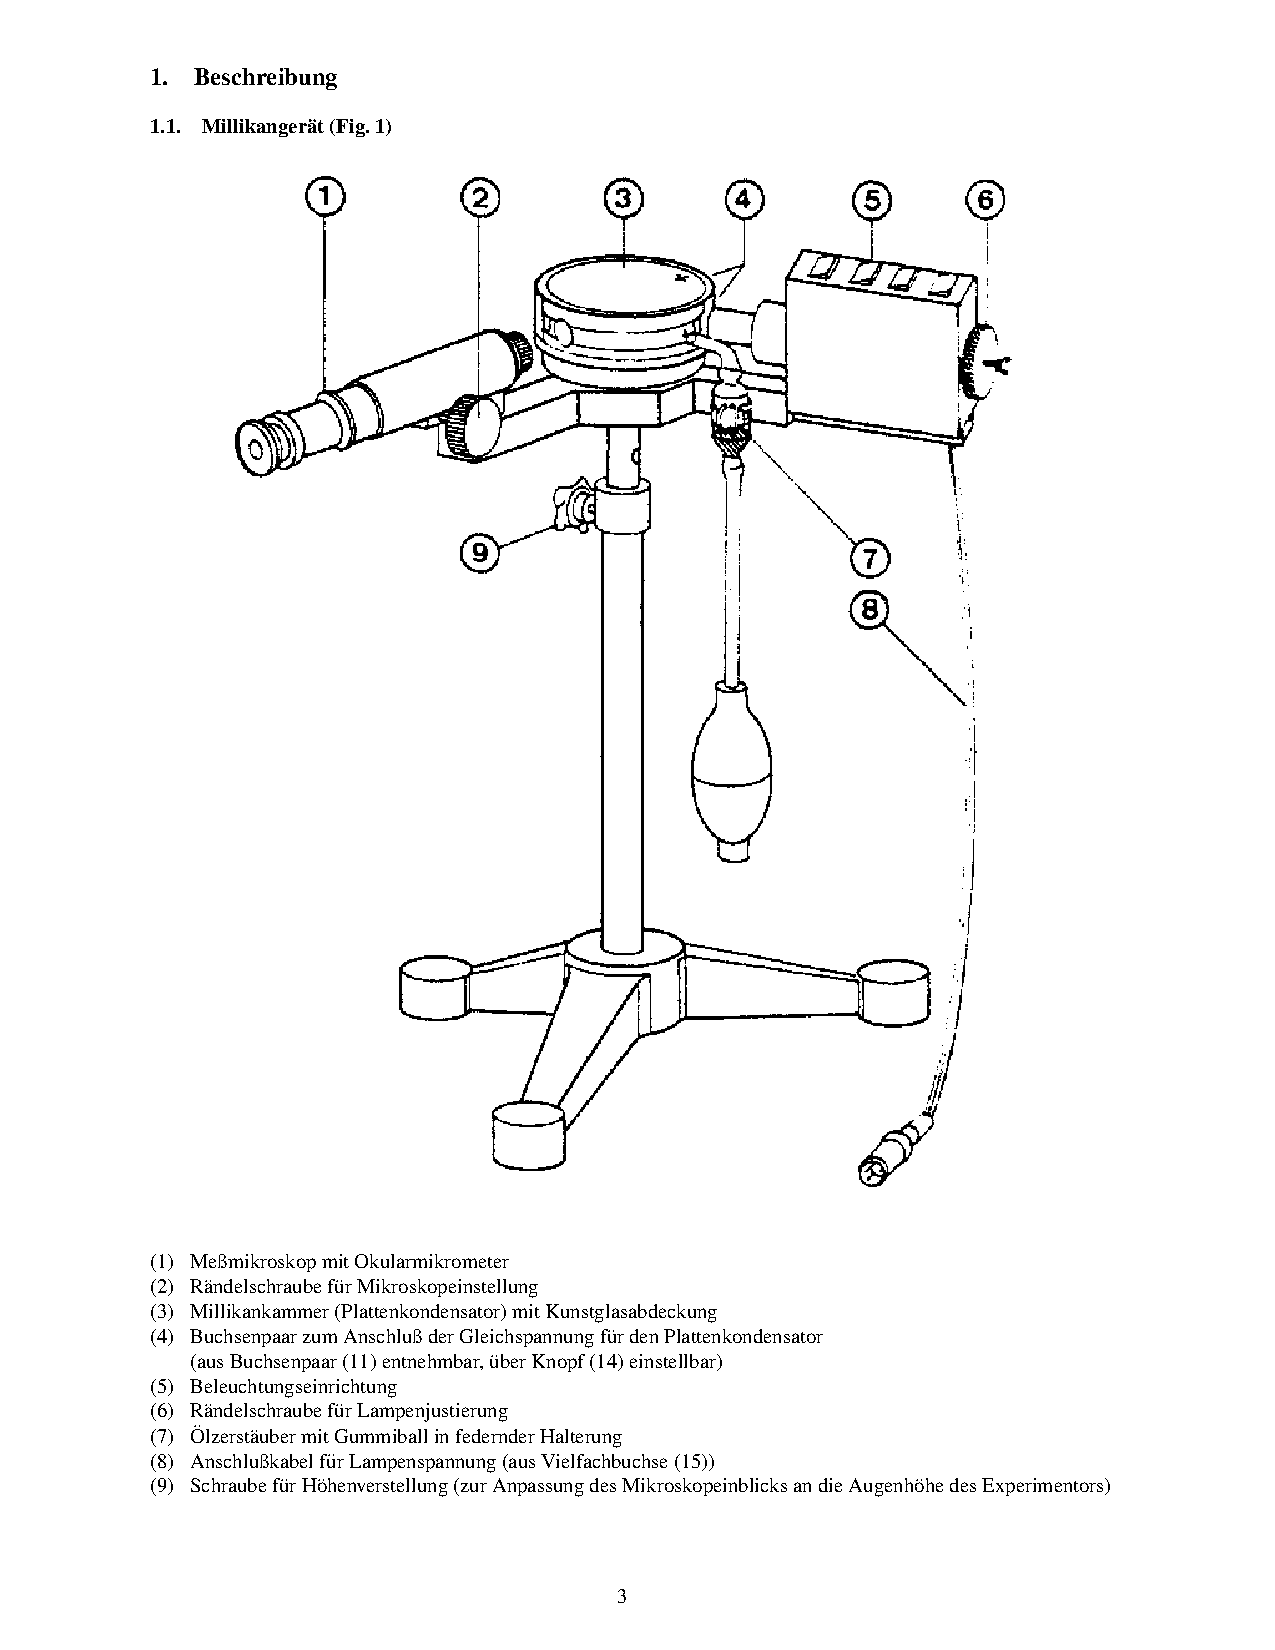
\includegraphics[trim = 10mm 75mm 10mm 10mm, clip, scale = 0.7]{aufbau.pdf}
  	\caption[Abbildung des Versuchsaufbaus]{Abbildung des Versuchsaufbaus\footnotemark}
  \label{fig:abb_versuch_3}
\end{figure}
\footnotetext{Abbildung entnommen von http://www.atlas.uni-wuppertal.de/~kind/ap22ap1\_millikan.pdf Seite 3 am 13.09.2014}

\begin{enumerate}
\item	Messmikroskop mit Okularmikrometer

\item	Rändelschraube für Mikroskopeinstellung

\item	Millikankammer (Plattenkondensator) mir Kunstglasabdeckung

\item	Buchsenpaar zum Anschluss der Gleichspannung für den Plattenkondensator

\item	Beleuchtungseinrichtung

\item	Rändelschraube für die Lampenjustierung

\item	Ölzerstäuber mit Gummiball in federnder Halterung

\item	Anschlusskabel für Lampenspannung

\item	Schraube für Höhenverstellung
\end{enumerate}

Durch den Ölzerstäuber wird Öl in die Kammer geblasen, die Tröpfchen, die sich dabei bilden werden mit der Lampe beleuchtet, wodurch die durch das Mikroskop gut zu sehen sind. Der Kondensator, der oben und unten an der Kammer anliegt ist mit einer Doppelstoppuhr verbunden, wodurch die Stoppuhr zeitgleich mit dem Kondensator getriggert wird.

\section{Versuchsdurchführung}


\subsection{Praktische Durchführung}
Mithilfe des Milikangerätes und zwei Stoppuhren bestimmen wir in diesem Versuch die Ladung einiger Öltröpfchen, welche im homogenen E-Feld eines Plattenkondensators zum schweben gebracht werden. Unsere Versuchsergebnisse sollen danach in einem Histogramm visualisiert werden.

\subsection{Theoretische Durchführung}
Die Ladung $Q$ eines Öltrößfchens bestimmen wir nach folgender Gleichung:
\begin{align}
Q = (v_1+v_2)\sqrt{\frac{v_1 \eta^3}{2\rho g}} \frac{18 \pi d}{U}
\end{align}
Dabei ist $\eta = 1,81\cdot10^{-5}\frac{Ns}{m^2}$ die Viskosität von Luft, $v_1$ die Fallgeschwindigkeit im Feldfreien Raum mit Stokessscher Reibungskraft, $v_2$ die Steiggeschwindigkeit der Öltröpfchen im homogenen E-Feld, $U$ die Spannung, die am Plattenkondensator anliegt, $\rho = 874 \frac{kg}{m^3}$ die Dichte von Öl abzüglich der Dichte von Luft, $g = 9,81 \frac{m}{s^2}$ die Erdbeschleunigung und $ d = 6\cdot10^{-3} m$ der Plattenabstand.\\
$v_1$ und $v_2$ bestimmen wir, da sie über die gemessene Strecke durch die Reibungskraft Konstant gehalten werden, über die mittlere Änderung:
\begin{align}
v = 1,875\frac{\Delta x}{\Delta t}
\end{align}
Der Vorfaktor 1,875 resultiert aus der Vergrößerung des Objektivs, wobei $x = n*10^{-4}m$ über die Anzahl der überstrichenen Skalenteile $n$ bestimmt wird.\\
Für den Fehler gilt:
\begin{align}
\delta_v = 1,875 \sqrt{
\left(\frac{\delta_{\Delta x}}{\Delta t}\right)^2+
\left(\frac{\Delta x}{(\Delta t)^2}\delta_{\Delta t}\right)^2}
\end{align}
Es ergibt sich folgende Rechnung:
\begin{align}
Q = (v_1+v_2)\frac{\sqrt{v_1}}{U}\cdot2\cdot10^{-10} \text{C}
\end{align}
Der Fehler berechnet sich durch:
\begin{align}
\delta_Q = \sqrt{
\left(\left(\frac{3 \sqrt{v_1}}{2 U} + \frac{v_2}{U2\sqrt{v_1}}
\right)\delta_{v_1}\right)^2+
\left(\frac{\sqrt{v_1}}{U}\delta_{v_2}\right)^2+
\left((v_1+v_2)\frac{\sqrt{v_1}}{U^2}\delta_{U}\right)^2}
\cdot2\cdot10^{-10}\text{C}
\end{align}
Da die Stokesreibung für Tröpfchen in der Größenordnung der mittleren freien Weglänge zwischen Luftmolekülen nicht mehr exakt gilt benutzen wir zum Schluss einen Korrekturfaktor für unsere Ladung, der in der Versuchsanleitung angegeben ist.\\
Wir berechnen unsere korrigierte Ladung $Q_k$ nach folgender Formel:
\begin{align}
Q_k = \frac{Q}{\left(1+\frac{b}{rp}\right)^{\frac{3}{2}}}
\label{eqn:q_r}
\end{align}
$ b = 6,33 \cdot \text{mbar m}$ ist dabei der aus der Versuchsbeschreibung entnommene Korrekturfaktor, $r$ der Radius des Öltröpfchens und $p$ der in mbar gemessene Druck.\\
Es ergibt sich damit ein Fehler von:
\begin{align}
\delta_{Q_k} = \sqrt{
\left(\frac{\delta_Q}{\left(1+\frac{b}{rp}\right)^{\frac{3}{2}}}\right)^2+
\left(\frac{3Q}{2\left(1+\frac{b}{rp}\right)^{\frac{5}{2}}}\frac{b}{rp^2}\delta_p\right)^2+
\left(\frac{3Q}{2\left(1+\frac{b}{rp}\right)^{\frac{5}{2}}}\frac{b}{r^2p}\delta_r\right)^2
}
\label{eqn:q_r_sigma}
\end{align}
Für diesen Korrekturfaktor muss zusätzlich der Radius des Öltröpfchen bekannt sein, sowie der Druck!
Den Radius $r$ der Öltröpfchen kann näherungsweise nach folgender Formel bestimmt werden, welche sich aus den Kräften ergibt:
\begin{align}
r = \sqrt{\frac{9\eta v_1}{2\rho g}}
\end{align}
Da wie bereits erwähnt die Kräfte mit einem Fehler behaftet sind, ist der so bestimmte Radius (gleiche Fehlerquelle wie bei der Ladung) ebenfalls etwas zu groß. Der Korrekturfaktor für die Viskosität ist jedoch vom Radius abhängig, sodass sich eine genauere Formel zur Berechnung des eigentlichen Radius, durch Einsetzen von 
\begin{align}
\eta_{\text{neu}} = \frac{\eta_{\text{alt}}}{1+\frac{b}{rp}}
\end{align} 
anstelle von $\eta = \eta_{alt}$ in die voherige Formel, ergibt:
\begin{align}
r_k = -\frac{b}{2p}+\sqrt{\frac{b^2}{4p^2}+\frac{9\eta v_1}{2\rho g}}
\end{align}
Der Fehler für den korrigierten Radius $r_k$ ergibt sich dann mit:
\begin{align}
\delta_{r_k} = \sqrt{
\left(\frac{b}{2p^2}\left(1+\frac{b}{p\sqrt{\frac{b^2}{p^2}+\frac{18\eta v_1}{\rho g}}}\right)\delta_p\right)^2+
\left(\frac{9\eta}{2\rho g\sqrt{\frac{b^2}{p^2}+\frac{18\eta v_1}{\rho g}}}\delta_{v_1}\right)^2}
\end{align}
\section{Messergebnisse}

\begin{table}[H]
\caption{Materialeigenschaften der Versuchsinstrumente. Der Druck wurde der Seite www.stadtnetz-wuppertal.de entnommen.}
\begin{center}
\begin{tabular}{|l|l|}
\hline
Druck/mbar & Fehler/mbar \\ \hline
\multicolumn{1}{|r|}{1018} & \multicolumn{1}{r|}{5} \\ \hline
B/mbar$\cdot$m & $\eta$/(Ns/m$^2$) \\ \hline
\multicolumn{1}{|r|}{6,33E-005} & \multicolumn{1}{r|}{1,81E-005} \\ \hline
d/m & $\rho_\text{Oel}$/(kg/m$^3$) \\ \hline
\multicolumn{1}{|r|}{6,00E-003} & \multicolumn{1}{r|}{875,3} \\ \hline
$\rho_\text{L}$/(kg/m$^3$) & $\rho$/(kg/m$^3$) \\ \hline
\multicolumn{1}{|r|}{1,29} & \multicolumn{1}{r|}{874} \\ \hline
\end{tabular}
\end{center}
\label{tab:messwerte_m}
\end{table}



\begin{table}[H]
\caption{Messdaten für den Sinkfall. Der Fehler von U wurde mit 1/V, der Fehler der Skaleneinheit mit 0,5, der Fehler von t\_1 mit 0,5/s und der Fehler von s\_1 mit 3E-005/m angenommen}
\begin{center}
\begin{tabular}{|r|r|r|r|r|r|r|}
\hline
\multicolumn{1}{|l|}{Nummer} & \multicolumn{1}{|l|}{U/V} & \multicolumn{1}{l|}{Skalenanteile\_1} & \multicolumn{1}{l|}{t\_1/s} & \multicolumn{1}{l|}{s\_1/m} & \multicolumn{1}{l|}{v\_1/(m/s)} & \multicolumn{1}{l|}{Fehler/(m/s)} \\ \hline
1 & 247 & 10,0 & 18,6 & 0,0005 & 2,9E-005 & 2E-006 \\ \hline
2 & 505 & 20,0 & 39,5 & 0,0011  & 2,70E-005 & 8E-007 \\ \hline
3 & 505 & 20,0 & 22,4 & 0,0011 & 2,7E-005  & 2E-006 \\ \hline
4 & 162 & 10,0 & 13 & 0,0005  & 4,1E-005 & 3E-006 \\ \hline
5 & 162 & 10,0 & 12,6 & 0,0005  & 4,2E-005 & 3E-006 \\ \hline
6 & 162 & 10,0 & 14,5 & 0,0005  & 3,7E-005 & 2E-006 \\ \hline
7 & 162 & 10,0 & 13,6 & 0,0005  & 3,9E-005 & 2E-006 \\ \hline
8 & 162 & 10,0 & 13,7 & 0,0005  & 3,9E-005 & 2E-006 \\ \hline
9 & 162 & 10,0 & 25,2 & 0,0005  & 2,11E-004 & 1E-006 \\ \hline
10 & 162 & 10,0 & 27 & 0,0005  & 2,0E-005 & 1E-006 \\ \hline
11 & 505 & 20,0 & 16,4 & 0,0011  & 6,0E-005 & 3E-006 \\ \hline
12 & 505 & 20,0 & 34,3 & 0,0011  & 3,11E-005 & 9E-007 \\ \hline
13 & 505 & 20,0 & 11,6 & 0,0011  & 9,2E-005 & 5E-006 \\ \hline
14 & 505 & 20,0 & 23,6 & 0,0011  & 4,5E-005 & 1E-006 \\ \hline
15 & 505 & 20,0 & 40,7 & 0,0011  & 2,62E-005 & 7E-007 \\ \hline
16 & 505 & 20,0 & 21,1 & 0,0011  & 5,1E-005 & 2E-006 \\ \hline
17 & 505 & 50,0 & 42,2 & 0,0027  & 6,3E-005 & 1E-006 \\ \hline
18 & 505 & 10,0 & 26,7 & 0,0005  & 2,0E-005 & 1E-006 \\ \hline
19 & 505 & 20,0 & 17,9 & 0,0011  & 6,0E-005 & 2E-006 \\ \hline
20 & 505 & 10,0 & 21,7 & 0,0005  & 2,5E-005 & 1E-006 \\ \hline
21 & 505 & 10,0 & 8,4 & 0,0005  & 6,3E-005 & 5E-006 \\ \hline
22 & 505 & 20,0 & 18,5 & 0,0011  & 5,8E-005 & 2E-006 \\ \hline
23 & 505 & 20,0 & 19,7 & 0,0011  & 5,4E-005 & 2E-006 \\ \hline
24 & 505 & 20,0 & 17,2 & 0,0011  & 6,2E-005 & 2E-006 \\ \hline
25 & 505 & 20,0 & 15,1 & 0,0011  & 7,1E-005 & 3E-006 \\ \hline
26 & 505 & 20,0 & 16 & 0,0011  & 6,7E-005 & 2E-006 \\ \hline
27 & 505 & 20,0 & 17,3 & 0,0011  & 6,1E-005 & 2E-006 \\ \hline
28  & 505 & 20,0 & 15,7 & 0,0011  & 6,8E-005 & 3E-006 \\ \hline
29 & 505 & 20,0 & 11,8 & 0,0011  & 9,0E-005 & 4E-006 \\ \hline
30 & 505 & 20,0 & 11,2 & 0,0011  & 9,5E-005 & 5E-006 \\ \hline
31 & 505 & 20,0 & 11,3 & 0,0011  & 9,4E-005 & 5E-006 \\ \hline
32 & 505 & 20,0 & 11,3 & 0,0011  & 9,4E-005 & 5E-006 \\ \hline
33 & 505 & 20,0 & 9,3 & 0,0011  & 1,1E-005 & 7E-006 \\ \hline
34 & 505 & 20,0 & 20,2 & 0,0011  & 5,3E-005 & 2E-006 \\ \hline
35 & 505 & 20,0 & 9,1 & 0,0011  & 1,1E-005 & 7E-006 \\ \hline
36 & 505 & 20,0 & 38,5 & 0,0011  & 2,77E-005 & 8E-007 \\ \hline
37 & 505 & 20,0 & 11,2 & 0,0011  & 9,5E-005 & 5E-006 \\ \hline
38 & 505 & 20,0 & 29,6 & 0,0011  & 3,6E-005 & 1E-006 \\ \hline
\end{tabular}
\end{center}
\label{tab:messwerte_1}
\end{table}


\begin{table}[H]
\caption{Messdaten für den Steigfall. Der Fehler der Skaleneinheit wurde mit 0,5, der Fehler von t\_2 mit 0,5/s und der Fehler von s\_2 mit  3E-005 angenommen.}
\begin{center}
\begin{tabular}{|r|r|r|r|r|r|}
\hline
\multicolumn{1}{|l|}{Nummer} & \multicolumn{1}{|l|}{Skalenanteile\_2} & \multicolumn{1}{l|}{t\_2/s} & \multicolumn{1}{l|}{s\_2/m} & \multicolumn{1}{l|}{v\_2/(m/s)} & \multicolumn{1}{l|}{Fehler/(m/s)} \\ \hline
1 & 10,0 & 10,9 & 0,0005 & 4,9E-005 & 3E-006 \\ \hline
2 & 20,0 & 14,4 & 0,0011 & 7,4E-005 & 3E-006 \\ \hline
3 & 20,0 & 45,8 & 0,0011 & 2,3E-005 & 6E-007 \\ \hline
4 & 10,0 & 30,9 & 0,0005 & 1,72E-005 & 9E-007 \\ \hline
5 & 10,0 & 13,7 & 0,0005 & 3,9E-005 & 2E-006 \\ \hline
6 & 10,0 & 26,3 & 0,0005 & 2,0E-005 & 1E-006 \\ \hline
7 & 10,0 & 26,7 & 0,0005 & 1,9E-005 & 1E-006 \\ \hline
8 & 10,0 & 28,9 & 0,0005 & 1,8E-005 & 1E-006 \\ \hline
9 & 10,0 & 40,3 & 0,0005 & 1,3E-005 & 7E-007 \\ \hline
10 & 10,0 & 23,7 & 0,0005 & 2,3E-005 & 1E-006 \\ \hline
11 & 20,0 & 19,8 & 0,0011 & 5,4E-005 & 2E-006 \\ \hline
12 & 20,0 & 28,4 & 0,0011 & 3,8E-005 & 1E-006 \\ \hline
13 & 20,0 & 7,2 & 0,0011 & 1,4E-004 & 1E-005 \\ \hline
14 & 20,0 & 13,5 & 0,0011 & 7,9E-005 & 4E-006 \\ \hline
15 & 20,0 & 5,9 & 0,0011 & 1,8E-004 & 1E-005 \\ \hline
16 & 20,0 & 44,8 & 0,0011 & 2,4E-005 & 7E-007 \\ \hline
17 & 20,0 & 20,9 & 0,0011 & 5,1E-005 & 2E-006 \\ \hline
18 & 10,0 & 2,2 & 0,0005 & 2,4E-004 & 6E-005 \\ \hline
19 & 20,0 & 76,9 & 0,0011 & 1,4E-005 & 4E-007 \\ \hline
20 & 10,0 & 2,7 & 0,0005 & 1,9E-004 & 4E-005 \\ \hline
21 & 10,0 & 4,5 & 0,0005 & 1,1E-004 & 1E-005 \\ \hline
22 & 20,0 & 72,9 & 0,0011 & 1,5E-005 & 4E-007 \\ \hline
23 & 20,0 & 76,3 & 0,0011 & 1,4E-005 & 46E-007 \\ \hline
24 & 20,0 & 8,7 & 0,0011 & 1,23E-004 & 8E-006 \\ \hline
25 & 20,0 & 8,6 & 0,0011 & 1,24E-004 & 8E-006 \\ \hline
26 & 20,0 & 8,7 & 0,0011 & 1,2E-005 & 8E-006 \\ \hline
27 & 20,0 & 9 & 0,0011 & 1,1E-005 & 7E-006 \\ \hline
28 & 20,0 & 8,4 & 0,0011 & 1,3E-005 & 8E-006 \\ \hline
29 & 20,0 & 17 & 0,0011 & 6E-005 & 2E-006 \\ \hline
30 & 20,0 & 18,1 & 0,0011 & 5,9E-005 & 2E-006 \\ \hline
31 & 20,0 & 17,8 & 0,0011 & 6,0E-005 & 2E-006 \\ \hline
32 & 20,0 & 17,5 & 0,0011 & 6,1E-005 & 2E-006 \\ \hline
33 & 20,0 & 55,9 & 0,0011 & 1,91E-005 & 5E-007 \\ \hline
34 & 20,0 & 60,9 & 0,0011 & 1,75E-005 & 5E-007 \\ \hline
35 & 20,0 & 45,4 & 0,0011 & 2,35E-005 & 6E-007 \\ \hline
36 & 20,0 & 12,9 & 0,0011 & 8,3E-005 & 4E-006 \\ \hline
37 & 20,0 & 85,2 & 0,0011 & 1,25E-005 & 3E-007 \\ \hline
38 & 20,0 & 20,8 & 0,0011 & 5,1E-005 & 2E-006 \\ \hline
\end{tabular}
\end{center}
\label{tab:messwerte_2}
\end{table}


\begin{table}[H]
\caption{Ergebnisse die aus den Messwerten bestimmt wurden, der Fehler des Radiuses ergab sich mit 2E-010}
\begin{center}
\begin{tabular}{|r|r|r|r|r|r|}
\hline
\multicolumn{1}{|l|}{Nummer} & \multicolumn{1}{|l|}{Radius/m} & \multicolumn{1}{l|}{Q/C} & \multicolumn{1}{l|}{Fehler/C} & \multicolumn{1}{l|}{Q\_k/C} & \multicolumn{1}{l|}{Fehler/C} \\ \hline
1 & 4,917E-007 & 3,4E-019 & 2E-020 & 2,814E-019 & 1,E-022 \\ \hline
2 & 4,764E-007 & 2,08E-019 & 9E-021 & 1,731E-019 & 1E-022 \\ \hline
3 & 6,422E-007 & 1,94E-019 & 8E-021 & 1,687E-019 & 2E-022 \\ \hline
4 & 0,594E-007 & 4,6E-019 & 4E-020 & 3,970E-019 & 2E-022 \\ \hline
5 & 6,038E-007 & 6,5E-019 & 5E-020 & 5,634E-019 & 2E-022 \\ \hline
6 & 5,608E-007 & 4,3E-019 & 3E-020 & 3,649E-019 & 1E-022 \\ \hline
7 & 5,801E-007 & 4,6E-019 & 3E-020 & 3,928E-019 & 2E-022 \\ \hline
8 & 5,778E-007 & 4,4E-019 & 3E-020 & 3,792E-019 & 2E-022 \\ \hline
9 & 4,184E-007 & 2,0E-019 & 1E-020 & 1,587E-019 & 1E-022 \\ \hline
10 & 4,032E-007 & 2,3E-019 & 1E-020 & 1,8698E-019 & 9E-023 \\ \hline
11 & 7,556E-007 & 3,8E-019 & 2E-020 & 3,373E-019 & 2E-022 \\ \hline
12 & 5,133E-007 & 1,51E-019 & 5E-021 & 1,277E-019 & 1E-022 \\ \hline
13 & 9,041E-007 & 9,1E-019 & 6E-020 & 8,253E-019 & 3E-022 \\ \hline
14 & 6,249E-007 & 3,3E-019 & 1E-020 & 2,869E-019 & 2E-022 \\ \hline
15 & 4,688E-007 & 4,2E-019 & 3E-020 & 3,482E-019 & 1E-022 \\ \hline
16 & 6,626E-007 & 2,09E-019 & 9E-021 & 1,830E-019 & 2E-022 \\ \hline
17 & 7,443E-007 & 3,60E-019 & 8E-021 & 3,188E-019 & 2E-022 \\ \hline
18 & 4,056E-007 & 5E-019 & 1E-019 & 3,7500E-019 & 9E-023 \\ \hline
19 & 7,219E-007 & 2,2E-019 & 1E-020 & 1,984E-019 & 2E-022 \\ \hline
20 & 4,531E-007 & 4,4E-019 & 8E-020 & 3,596E-019 & 1E-022 \\ \hline
21 & 7,461E-007 & 5,7E-019 & 6E-020 & 5,094E-019 & 2E-022 \\ \hline
22 & 7,097E-007 & 2,2E-019 & 1E-020 & 1,917E-019 & 2E-022 \\ \hline
23 & 6,868E-007 & 1,99E-019 & 9E-021 & 1,743E-019 & 2E-022 \\ \hline
24 & 7,371E-007 & 5,8E-019 & 3E-020 & 5,099E-019 & 2E-022 \\ \hline
25 & 7,887E-007 & 6,5E-019 & 3E-020 & 5,783E-019 & 2E-022 \\ \hline
26 & 7,653E-007 & 6,1E-019 & 3E-020 & 5,444E-019 & 2E-022 \\ \hline
27 & 7,347E-007 & 5,6E-019 & 3E-020 & 4,960E-019 & 2E-022 \\ \hline
28 & 7,729E-007 & 6,4E-019 & 3E-020 & 5,666E-019 & 2E-022 \\ \hline
29 & 8,961E-007 & 5,8E-019 & 3E-020 & 5,214E-019 & 3E-022 \\ \hline
30 & 9,206E-007 & 6,0E-019 & 4E-020 & 5,402E-019 & 3E-022 \\ \hline
31 & 9,164E-007 & 5,9E-019 & 3E-020 & 5,381E-019 & 3E-022 \\ \hline
32 & 9,164E-007 & 6,0E-019 & 3E-020 & 5,417E-019 & 3E-022 \\ \hline
33 & 1,013E-006 & 5,7E-019 & 5E-020 & 5,189E-019 & 4E-022 \\ \hline
34 & 6,779E-007 & 2,0E-019 & 9E-021 & 1,774E-019 & 2E-022 \\ \hline
35 & 1,025E-006 & 6,0E-019 & 4E-020 & 5,523E-019 & 4E-022 \\ \hline
36 & 4,829E-007 & 2,3E-019 & 9E-021 & 1,919E-019 & 1E-022 \\ \hline
37 & 9,206E-007 & 4,2E-019 & 3E-020 & 3,776E-019 & 3E-022 \\ \hline
38 & 5,548E-007 & 2,1E-019 & 7E-021 & 1,770E-019 & 1E-022 \\ \hline
\end{tabular}
\end{center}
\label{tab:messwerte_3}
\end{table}


\section{Auswertung}
Bei dem Versuch sollt die Elementarladung und ihre Quantisierung gezeigt und bestimmt werden. Dazu wurde nach Gleichung \ref{eqn:q_r} die korrigierten Ladung der Öltröpfchen bestimmt, der Fehler ergibt sich nach Gleichung \ref{eqn:q_r_sigma}. Aus den bestimmten Ladungen wurde ein Histogramm erstellt (Wert aus Tabelle \ref{tab:messwerte_3}).

\begin{figure}[H] 
  \centering
    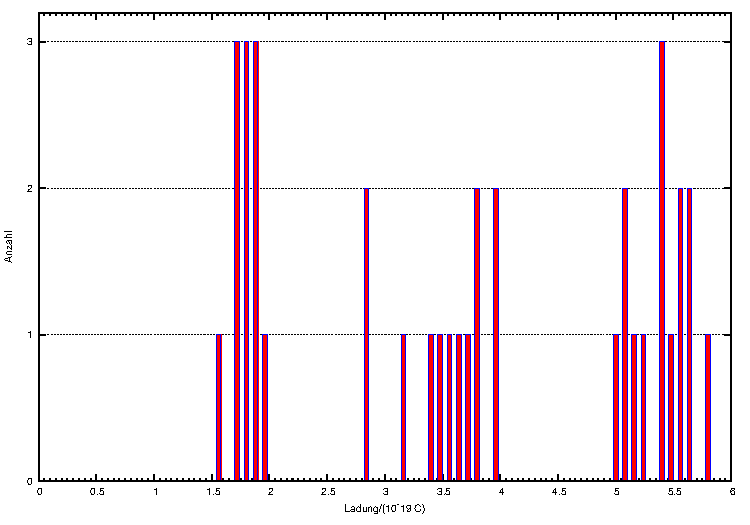
\includegraphics[scale = 1.3]{messung.pdf}
  	\caption[Histogramm der korrigierten Ladungen]{Histogramm der korrigierten Ladungen}
  \label{fig:histogramm}
\end{figure}

Aus dem Histogramm werden die drei Mittelwerte für die Quantisierung der Ladung gebildet.Dabei ergaben sich die folgenden Mittelwerte, n=1 \hspace*{4px} 1,8$(\pm0,1)\cdot 10^{-19}$C, n=2 \hspace*{4px} 3,5$(\pm 0,4)\cdot 10^{-19}$ und n=3 \hspace*{4px} 5,5$(\pm 0,2)\cdot 10^{-19}$C, die Fehler wurden dabei durch die Standartabweichung bestimmt. Bestimmt aus den Werten von n=2,3 die Elementarladung ergibt sich für n=2 einen Elementarladung von 1,8$(\pm 0,2)\cdot 10^{-19}$C und für n=3 \hspace*{4px} 1,82$(\pm 0,06)\cdot 10^{-19}$C

\section{Diskussion}
Erwartet wurde ein Wert von 1,62$\cdot 10^{-19}$C unser Wert liegt bei 1,8$\cdot 10^{-19}$C dies kommt wahrscheinlich an dem verwendetem Korrekturfaktor. Bei der geringen Anzahl an Messungen, die wir durchgeführt haben, lässt sich kein eigener Korrekturfaktor bestimmte, dazu wären viel mehr Messungen nötig gewesen. Jedoch sind unsere Messergebnisse in sich konsistent, da die aus den drei bestimmten Werte für die Elementarladung in den Fehlerbereichen der jeweils anderen Werte liegen.

\section{Fazit}
Der Versuch ist insgesamt gelungen, auch wenn der für die Elementarladung bestimmte Wert vom Literaturwert abweicht, so wurde doch deutlich gezeigt das Ladung in Diskreten Größen auftritt, welchen ein Vielfaches der Elementarladung sind.
 %Werte stimmen mit den Formeln überein/nicht überein

\end{document}

